\section{Python環境の構築手順}\label{sec: Python環境の構築手順}
本節ではデータ解析プラットフォームAnacondaの導入手順を説明する.
AnacondaはPythonのディストリビューションの一つであり,
その最大の特徴はデータ解析に有用な追加パッケージを多数そろえていることにある.
また,それらのパッケージの間の依存関係を処理するために
独自のパッケージ管理システムCondaが用意されていることも特徴の一つである.
Condaを用いることで,パッケージの導入・アップデート・削除のほか,
Python仮想環境の構築・管理なども容易に行うことが可能となる\footnote{%
この辺りの詳細については
公式ドキュメント
(\url{http://conda.pydata.org/docs/index.html})
などを参照されたい.
}.


\subsection{Windowsの場合}


\subsubsection{新規インストール}
\begin{enumerate}
\item
公式サイトのダウンロードページ
(\url{https://www.continuum.io/downloads/})
から自分のWindows環境($32$ビット版/$64$ビット版)\footnote{%
コントロールパネルから[システム]を開き,「システムの種類」で確認可能.
}に合ったインストーラをダウンロードする.
\item
ダウンロードしたインストーラを実行し,
表示された指示に従ってインストールする.
\end{enumerate}

\begin{attention}
ほかのPythonディストリビューション(ActivePythonなど)が
インストールされている場合,
Anacondaをインストールしても,
設定によっては前者が優先的に使用されてしまう.
優先順位を確認するためには,
コマンドプロンプト(cmd.exe)上で次のコマンドを実行すればよい.
\begin{lstlisting}[style=cmdline]
> where python.exe
\end{lstlisting}
このコマンドの出力の先頭行にAnaconda以外のPythonが表示されたときは,
以下の手順で
AnacondaのPythonが優先的に使用されるように変更する.
\begin{enumerate}
\item
コントロールパネルから
[システム]→[システムの詳細設定]→[環境変数]と進み,
システム環境変数の「Path」を選択して[編集]ボタンを押す.
\item
変数値からAnaconda関係のエントリを切り取り,
ほかのPythonディストリビューションに関するエントリより前に貼り付ける.
\item
[OK]ボタンを押して設定を保存・反映させる.
\end{enumerate}
\end{attention}

\begin{attention}
Cygwin Terminal上では
Windowsの「Path」の前に\verb|/usr/local/bin:/usr/bin|が自動で追加され,
CygwinのPythonが優先的に使用されてしまう.
Cygwin Terminal上でも
デフォルトでAnacondaのPythonが使用されるようにするためには,
Cygwin Terminal上でさらに次のコマンドを実行する.
\begin{lstlisting}[style=cmdline]
$ echo 'export PATH=<Anaconda directory>:$PATH' >> ~/.bashrc
$ echo "alias python='python -i'" >> ~/.bashrc
\end{lstlisting}
%Cygwin TerminalからAnacondaのPythonを呼び出す際には,
%\verb|cygstart|コマンドを使用して次のようにすべきであろう.
%\begin{lstlisting}[style=cmdline]
%$ cygstart <Anaconda directory>/python
%\end{lstlisting}
ここで,\verb|<Anaconda directory>|には
AnacondaのインストールディレクトリをCygwin形式で記入すること
(例えば\verb|/cygdrive/c/Anaconda3|).
Cygwin Terminalを開きなおせば,
AnacondaのPythonが優先されるようになっているはずである.
\end{attention}


\subsubsection{旧バージョンからのアップデート}
コマンドプロンプト(cmd.exe)を開き,以下の手続きを実行する.
\begin{enumerate}
\item
パッケージ管理システム自体をアップデートする.
\begin{lstlisting}[style=cmdline]
> conda update conda
\end{lstlisting}
\item
パッケージ群をアップデートする.
\begin{lstlisting}[style=cmdline]
> conda update anaconda
\end{lstlisting}
\end{enumerate}


\subsection{Mac OS Xの場合}
\begin{attention}
Mac OS Xに関しては,
公式インストーラを用いてAnacondaを導入したところ
Condaがほかのパッケージ管理システムと衝突した,
という事例が報告されている.
そこで,よりクリーンな導入方法として,
ここでは
パッケージ管理システムHomebrewとPythonバージョン管理ツールpyenvとを用いた
方法を紹介する.
\end{attention}


\subsubsection{新規インストール}
ターミナル(Bash\footnote{%
ターミナルとしてBash以外を使用している場合は
コマンドを適当に変更すること.
})を開き,以下の手続きを実行する.
\begin{enumerate}
\item
(OSをEl Capitanより前のバージョンからEl Capitan以降にアップデートした場合)
\verb|/usr/local|のパーミッションが書き換えられてしまっている可能性がある.
以下のコマンドでパーミッションを復元する.
\begin{lstlisting}[style=cmdline]
$ sudo chown -R $(whoami):admin /usr/local
\end{lstlisting}
\item
(プロキシを介してインターネットを利用している場合)
環境変数でプロキシを指定する.
\begin{lstlisting}[style=cmdline]
$ export http_proxy=http://<proxyhost>:<proxyport>
$ export https_proxy=https://<proxyhost>:<proxyport>
\end{lstlisting}
ここで,\verb|<proxyhost>|にはプロキシのURL,
\verb|<proxyport>|にはプロキシのポート番号を記入すること.
\item
\begin{description}[font=\normalfont,style=sameline]
\item[(Homebrewがインストールされていない場合)]
\leavevmode
\begin{enumerate}[(i)]
\item
Command Line Tools for Xcodeをインストールする.
\begin{lstlisting}[style=cmdline]
$ xcode-select --install
\end{lstlisting}
\item
Homebrewをインストールする\footnote{%
Xcodeのライセンスに同意していないことで警告が出た場合,
表示された指示に従ってライセンスに同意する.
}.
\begin{comment}
\begin{lstlisting}[style=cmdline]
$ ruby -e "$(curl -fsSL \
	https://raw.githubusercontent.com\
		/Homebrew/install/master/install)"
\end{lstlisting}
\end{comment}
\begin{comment}
\begin{lstlisting}[%
	style=cmdline,%
	escapechar=|]
$ ruby -e "$(curl|\textvisiblespace|-fsSL|\textvisiblespace|\
> https://raw.githubusercontent.com\
> /Homebrew/install/master/install)"
\end{lstlisting}
\end{comment}
\begin{lstlisting}[style=cmdline]
$ ruby -e "$(curl -fsSL https://raw.githubusercontent.com\
  /Homebrew/install/master/install)"
\end{lstlisting}
\end{enumerate}
\item[(Homebrewがすでにインストールされている場合)]
\leavevmode\\
Homebrew自体とパッケージ一覧をアップデートしたうえで,
全パッケージをアップデートする.
\begin{lstlisting}[style=cmdline]
$ brew update
$ brew upgrade
\end{lstlisting}
\end{description}
\item
Homebrewを用いてpyenvをインストールする.
\begin{comment}
\begin{lstlisting}[style=cmdline]
$ brew install pyenv
$ echo 'export PYENV_ROOT=/usr/local/var/pyenv' \
	>> ~/.bash_profile
$ echo 'eval "$(pyenv init -)"' >> ~/.bash_profile
$ source ~/.bash_profile
\end{lstlisting}
\end{comment}
\begin{comment}
\begin{lstlisting}[style=cmdline]
$ brew install pyenv
$ echo 'export PYENV_ROOT=/usr/local/var/pyenv' \
> >> ~/.bash_profile
$ echo 'eval "$(pyenv init -)"' >> ~/.bash_profile
$ source ~/.bash_profile
\end{lstlisting}
\end{comment}
\begin{lstlisting}[style=cmdline]
$ brew install pyenv
$ echo 'export PYENV_ROOT=/usr/local/var/pyenv' \
  >> ~/.bash_profile
$ echo 'eval "$(pyenv init -)"' >> ~/.bash_profile
$ source ~/.bash_profile
\end{lstlisting}
\item\label{enum: Mac OS Xへの新規インストール - Anacondaのインストール}
\begin{enumerate}[(i)]
\item
pyenvで導入可能なAnacondaのバージョン一覧を確認する.
\begin{lstlisting}[style=cmdline]
$ pyenv install --list | grep 'anaconda3'
\end{lstlisting}
\item
pyenvを用いてAnacondaをインストールし,
さらにデフォルトのPython環境として設定する.
\begin{lstlisting}[style=cmdline]
$ pyenv install anaconda3-<Anaconda version>
$ pyenv global anaconda3-<Anaconda version>
$ pyenv rehash
\end{lstlisting}
ここで,\verb|<Anaconda version>|には
インストールしたいAnacondaのバージョンを記入すること.
特に理由がなければ
最新版(2016年7月21日の時点では\verb|4.0.0|)
を指定すればよい.
\end{enumerate}
\end{enumerate}


\subsubsection{旧バージョンからのアップデート}
ターミナル(Bash)を開き,以下の手続きを実行する.
\begin{enumerate}
\item
(OSをEl Capitanより前のバージョンからEl Capitan以降にアップデートした場合)
\verb|/usr/local|のパーミッションが書き換えられてしまっている可能性がある.
以下のコマンドでパーミッションを復元する.
\begin{lstlisting}[style=cmdline]
$ sudo chown -R $(whoami):admin /usr/local
\end{lstlisting}
\item
(プロキシを介してインターネットを利用している場合)
環境変数でプロキシを指定する.
\begin{lstlisting}[style=cmdline]
$ export http_proxy=http://<proxyhost>:<proxyport>
$ export https_proxy=https://<proxyhost>:<proxyport>
\end{lstlisting}
ここで,\verb|<proxyhost>|にはプロキシのURL,
\verb|<proxyport>|にはプロキシのポート番号を記入すること.
\item
Homebrew自体とパッケージ一覧をアップデートしたうえで,
全パッケージをアップデートする.
\begin{lstlisting}[style=cmdline]
$ brew update
$ brew upgrade
\end{lstlisting}
\item
pyenvを用いて
最新バージョンのAnacondaを新規インストールする.
(手順については新規インストールの
ステップ\ref{enum: Mac OS Xへの新規インストール - Anacondaのインストール}を
参照.)
\item
(必要に応じて)旧バージョンをアンインストールする.
\begin{enumerate}[(i)]
\item
インストールされているAnacondaのバージョン一覧を確認する.
\begin{lstlisting}[style=cmdline]
$ pyenv versions
\end{lstlisting}
\item
pyenvを用いてAnacondaをアンインストールする.
\begin{lstlisting}[style=cmdline]
$ pyenv uninstall anaconda3-<Anaconda version>
\end{lstlisting}
ここで,\verb|<Anaconda version>|には
アンインストールしたいAnacondaのバージョンを記入すること.
\end{enumerate}
\end{enumerate}


\subsection{動作テストのためのサンプルコード}
動作テストのために,
コード\ref{code: 動作テストのためのサンプルコード}にサンプルコードを掲載する.
実行すれば
(実行方法については第\ref{sec: Jupyter Notebookの使い方}節を参照)
図\ref{fig: サンプルコードの実行結果}のような結果が得られるはずである.

\lstinputlisting[%
	style=python,%
	label={code: 動作テストのためのサンプルコード},%
	caption={動作テストのためのサンプルコード.矩形波に対する三角多項式近似をプロットする.}]{code/sample.py}

\begin{figure}[htbp]
\centering
\setlength{\fboxsep}{0pt}
\fcolorbox{gray}{gray}{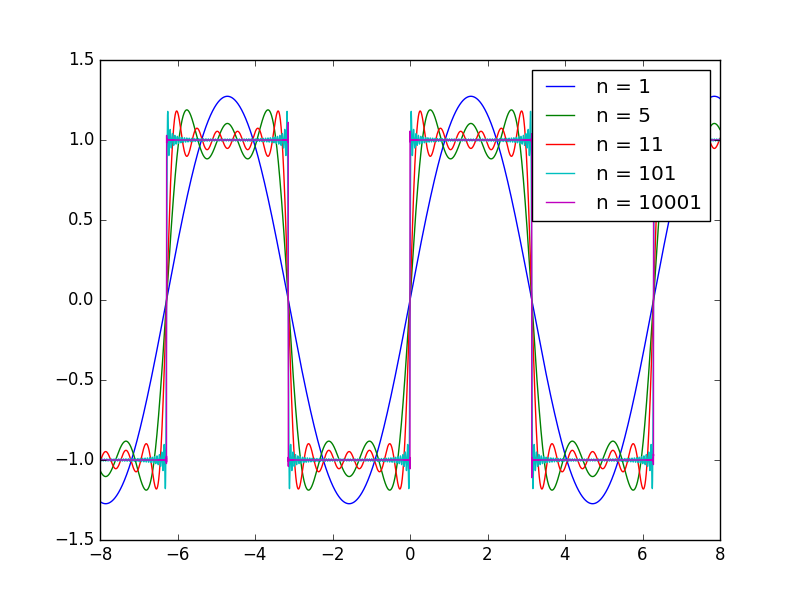
\includegraphics[scale=.4]{graphics/sample.png}}
\caption{\label{fig: サンプルコードの実行結果}%
コード\ref{code: 動作テストのためのサンプルコード}の実行結果.
}
\end{figure}
